%!TEX root = ../thesis.tex

\chapter{Налаштування системи Ethereum}
\label{chap:review}  %% відмічайте кожен розділ певною міткою -- на неї наприкінці необхідно посилатись

Для налаштування приватної ноди мережі Ethereum на основі протоколу Proof-Of-Work (PoW) з використанням Geth, будемо використовувати PoW алгоритм --- Ethash. Цей протокол є останньою версією алгоритму Dagger-Hashimoto, який використовується для майнінгу.

\section{Запуск та налаштування приватної ноди}

Спочатку встановимо geth:
\begin{verbatim}
sudo add-apt-repository -y ppa:ethereum/ethereum
sudo apt-get update
sudo apt-get install geth
\end{verbatim}

Тепер створимо директорію для нод:
\begin{verbatim}
mkdir -p ~/eth-private-node/{node1,node2,shared}
\end{verbatim}

Далі створимо два облікових записи:
\begin{verbatim}
geth --datadir ~/eth-private-node/node1 account new
\end{verbatim}

\vspace{-0.5cm}

\begin{figure}[ht]
        \centering
        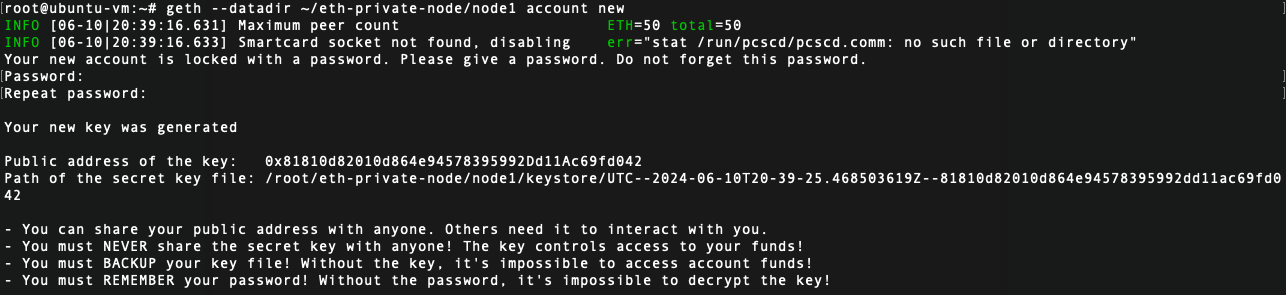
\includegraphics[scale=0.35]{IMAGES/newAcc1.png}
        % \caption{Количество круговых диаграмм, похожих на Пэкмена}
        \label{fig_pacman}
\end{figure}

Для 1-го акаунту отримали: \\
\textbf{Public address of the key:}   \texttt{0x81810d82010d864e94578395992Dd11Ac69fd042}

\newpage
\begin{verbatim}
geth --datadir ~/eth-private-node/node2 account new
\end{verbatim}

\vspace{-0.5cm}

\begin{figure}[ht]
        \centering
        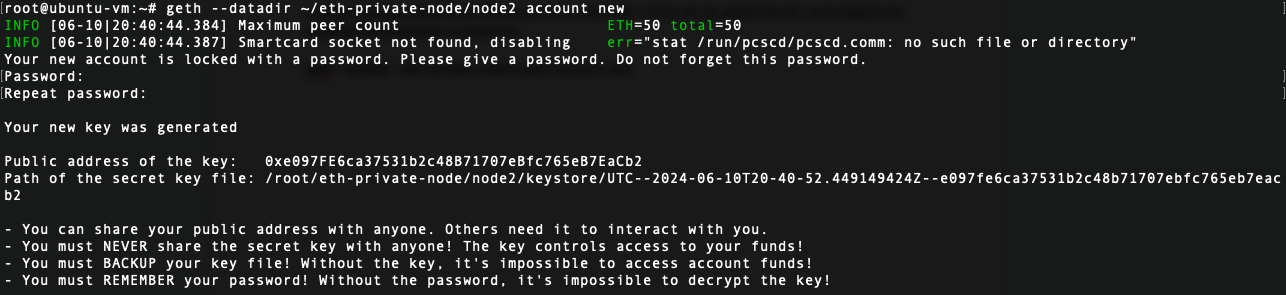
\includegraphics[scale=0.35]{IMAGES/newAcc2.png}
        % \caption{Количество круговых диаграмм, похожих на Пэкмена}
        \label{fig_pacman}
\end{figure}

Для 2-го акаунту отримали: \\
\textbf{Public address of the key:}   \texttt{0xe097FE6ca37531b2c48B71707eBfc765eB7EaCb2}

\vspace{0.5cm}
Створимо файл \texttt{genesis.json} у директорії \texttt{\~/eth-poa/shared}:
\begin{verbatim}
nano ~/eth-private-node/shared/genesis.json
\end{verbatim}

з наступним вмістом:

\vspace{-0.5cm}

\begin{figure}[ht]
        \centering
        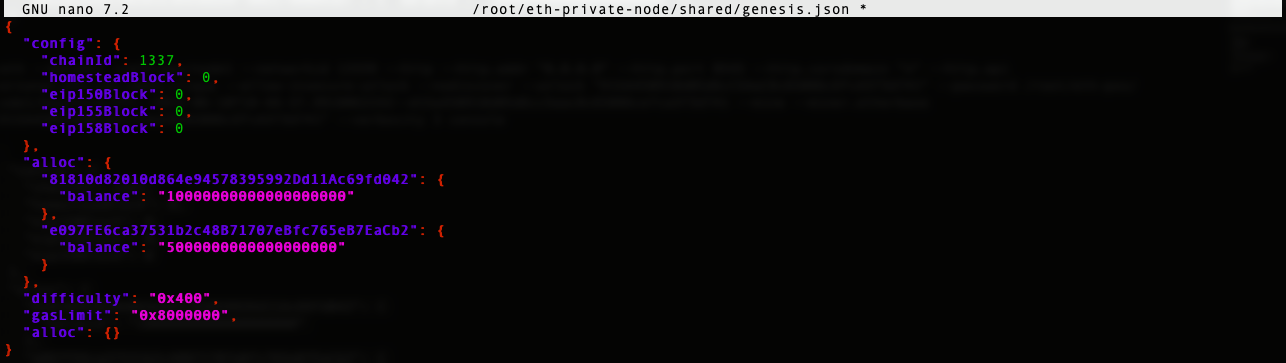
\includegraphics[scale=0.35]{IMAGES/genesis.png}
        % \caption{Количество круговых диаграмм, похожих на Пэкмена}
        \label{fig_pacman}
\end{figure}

Тепер переглянемо, що маємо в нашій структурі папки ноди:
\begin{verbatim}
tree -L 3
\end{verbatim}

\vspace{-0.5cm}

\begin{figure}[ht]
        \centering
        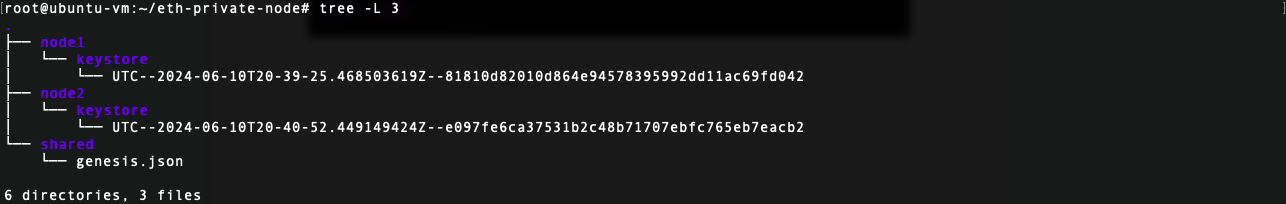
\includegraphics[scale=0.35]{IMAGES/tree.png}
        % \caption{Количество круговых диаграмм, похожих на Пэкмена}
        \label{fig_pacman}
\end{figure}

\newpage
Далі ініціалізуємо ноди.

Ініціалізуємо першу ноду з genesis-файлом:
\begin{verbatim}
geth --datadir ~/eth-private-node/node1 init 
~/eth-private-node/shared/genesis.json
\end{verbatim}

\vspace{-0.5cm}

\begin{figure}[ht]
        \centering
        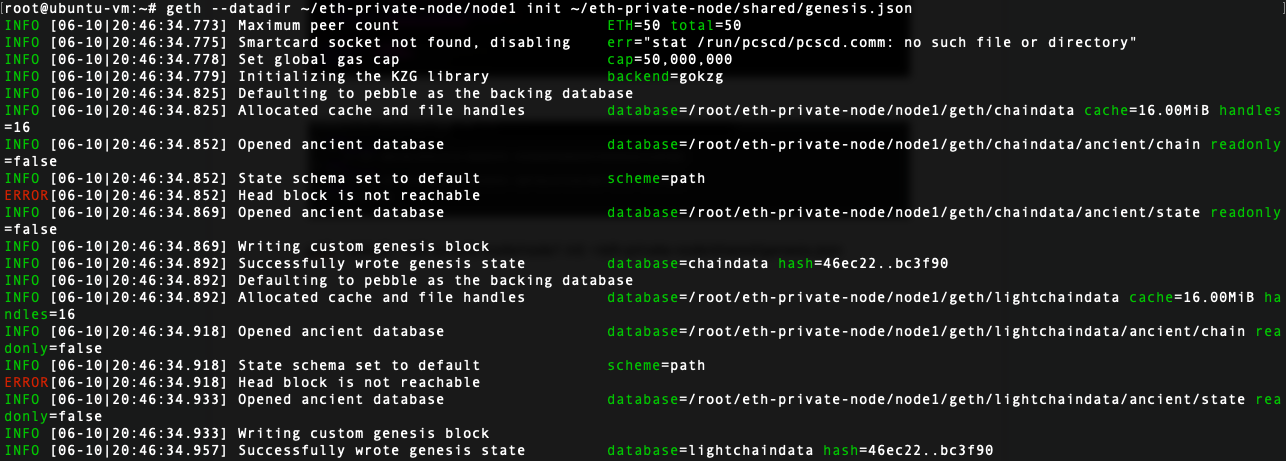
\includegraphics[scale=0.35]{IMAGES/init1.png}
        % \caption{Количество круговых диаграмм, похожих на Пэкмена}
        \label{fig_pacman}
\end{figure}

Ініціалізуємо другу ноду з genesis-файлом:
\begin{verbatim}
geth --datadir ~/eth-private-node/node2 init 
~/eth-private-node/shared/genesis.json
\end{verbatim}

\vspace{-0.5cm}

\begin{figure}[ht]
        \centering
        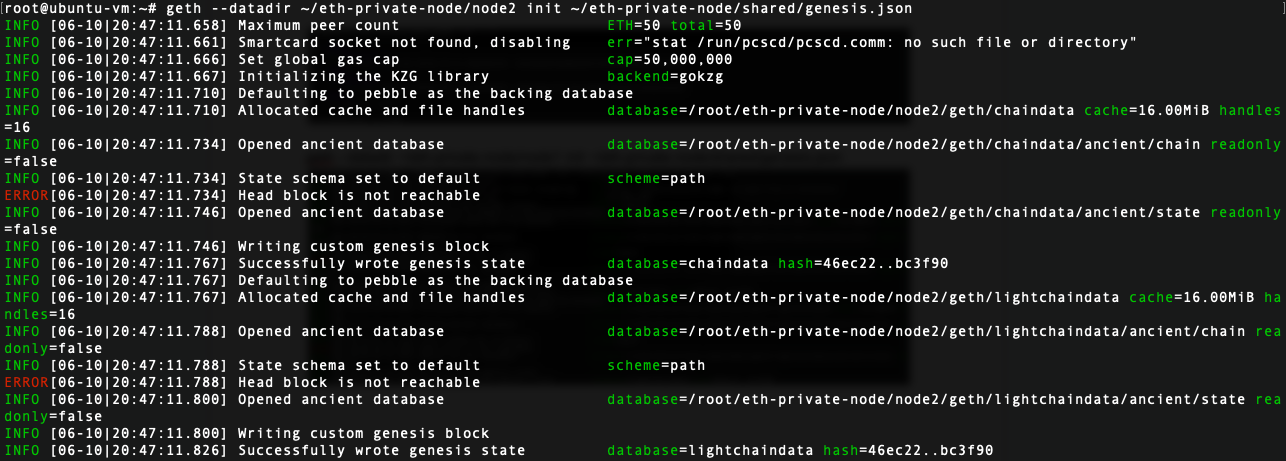
\includegraphics[scale=0.35]{IMAGES/init2.png}
        % \caption{Количество круговых диаграмм, похожих на Пэкмена}
        \label{fig_pacman}
\end{figure}

\newpage
Тепер запустимо першу ноду в ролі валідатора:
\begin{verbatim}
geth --datadir ~/eth-private/node1 --http --http.addr "0.0.0.0" 
--http.port 8545 --http.api "eth,net,web3,personal" 
--nodiscover console
\end{verbatim}

\vspace{-0.45cm}
\begin{figure}[ht]
        \centering
        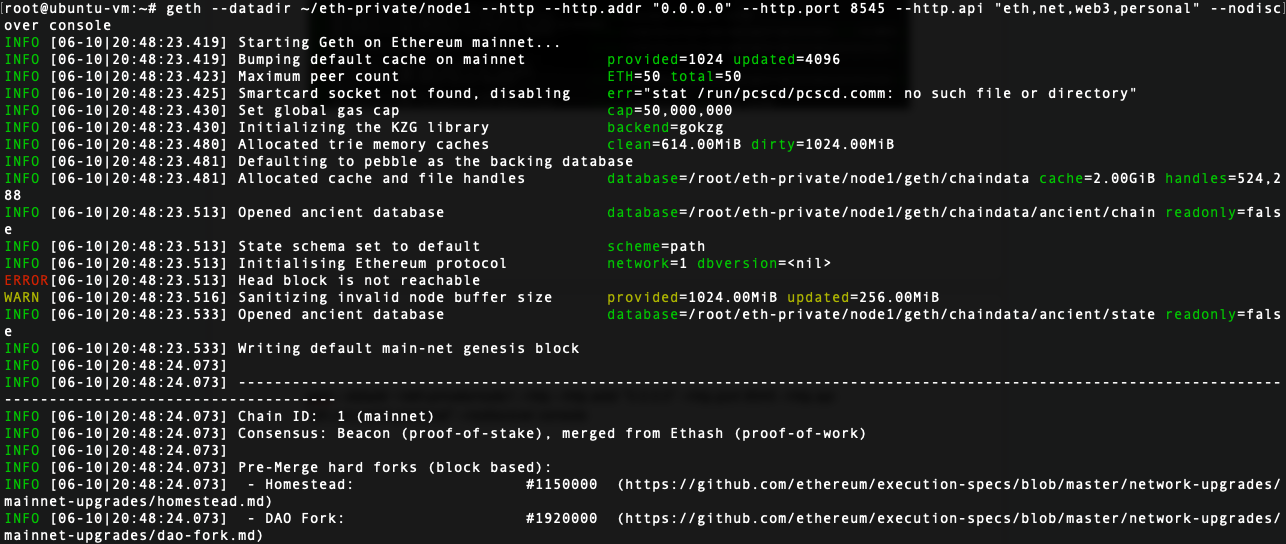
\includegraphics[scale=0.35]{IMAGES/launch11.png}
        % \caption{Количество круговых диаграмм, похожих на Пэкмена}
        \label{fig_pacman}
\end{figure}
\vspace{-1.35cm}
\begin{figure}[ht]
        \centering
        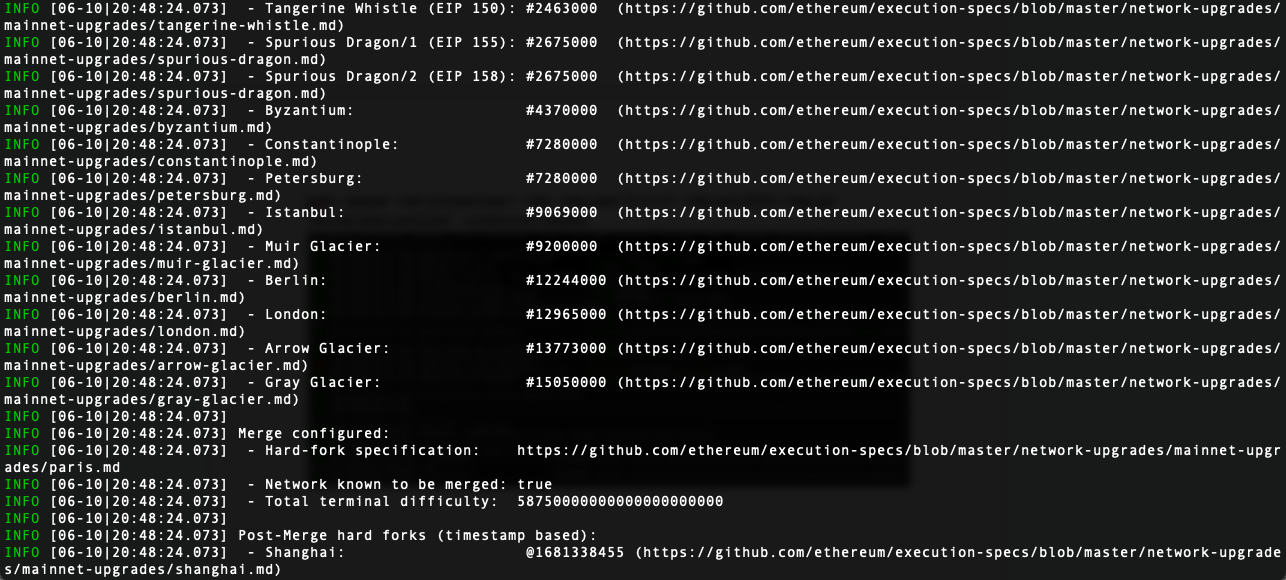
\includegraphics[scale=0.35]{IMAGES/launch12.png}
        % \caption{Количество круговых диаграмм, похожих на Пэкмена}
        \label{fig_pacman}
\end{figure}
\vspace{-1.35cm}
\begin{figure}[h!]
        \centering
        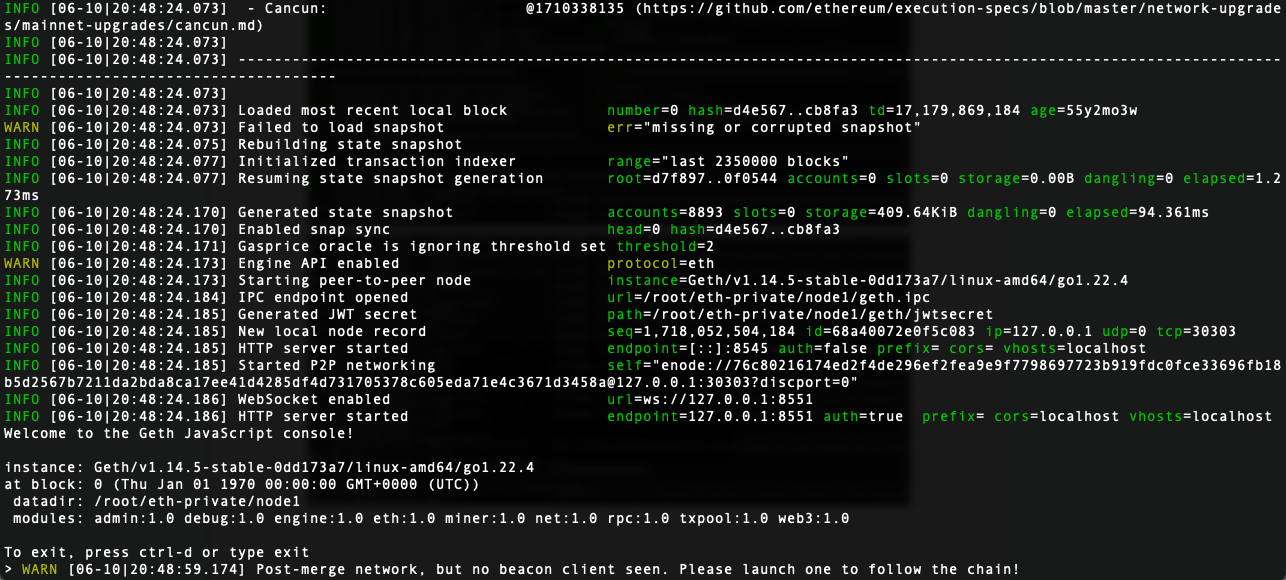
\includegraphics[scale=0.35]{IMAGES/launch13.png}
        % \caption{Количество круговых диаграмм, похожих на Пэкмена}
        \label{fig_pacman}
\end{figure}

\newpage
Тепер запустимо другу ноду та підключимо її до першої як до бут-ноди.
Для цього спочатку отримаємо enode першої ноди:
\begin{verbatim}
admin.nodeInfo.enode
\end{verbatim}

\vspace{-0.5cm}

\begin{figure}[ht]
        \centering
        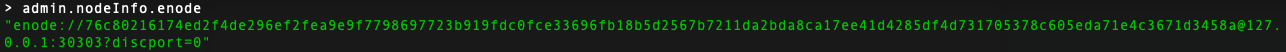
\includegraphics[scale=0.35]{IMAGES/enode.png}
        % \caption{Количество круговых диаграмм, похожих на Пэкмена}
        \label{fig_pacman}
\end{figure}

Далі запустимо другу ноду, вказавши enode першої ноди:
\begin{verbatim}
geth --datadir ~/eth-private/node2 --http --http.addr "0.0.0.0" 
--http.port 8552 --http.api "eth,net,web3,personal" --bootnodes
"enode://76c8021617.." --nodiscover --port 30304 console
\end{verbatim}

\vspace{-0.5cm}

\begin{figure}[ht]
        \centering
        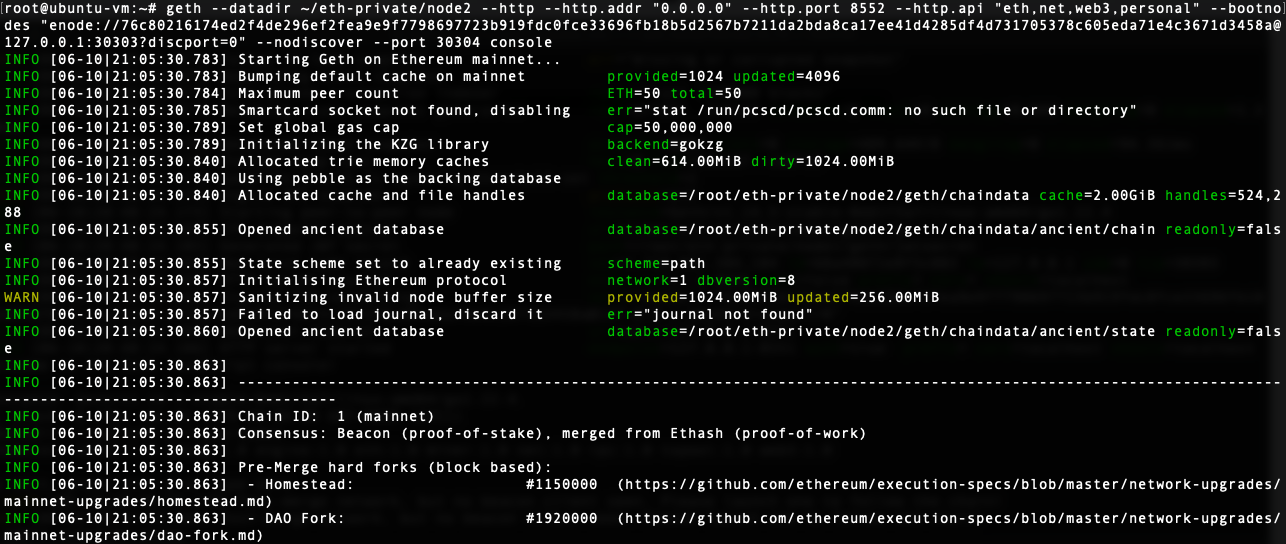
\includegraphics[scale=0.35]{IMAGES/launch21.png}
        % \caption{Количество круговых диаграмм, похожих на Пэкмена}
        \label{fig_pacman}
\end{figure}
\vspace{-1cm}
\begin{figure}[ht]
        \centering
        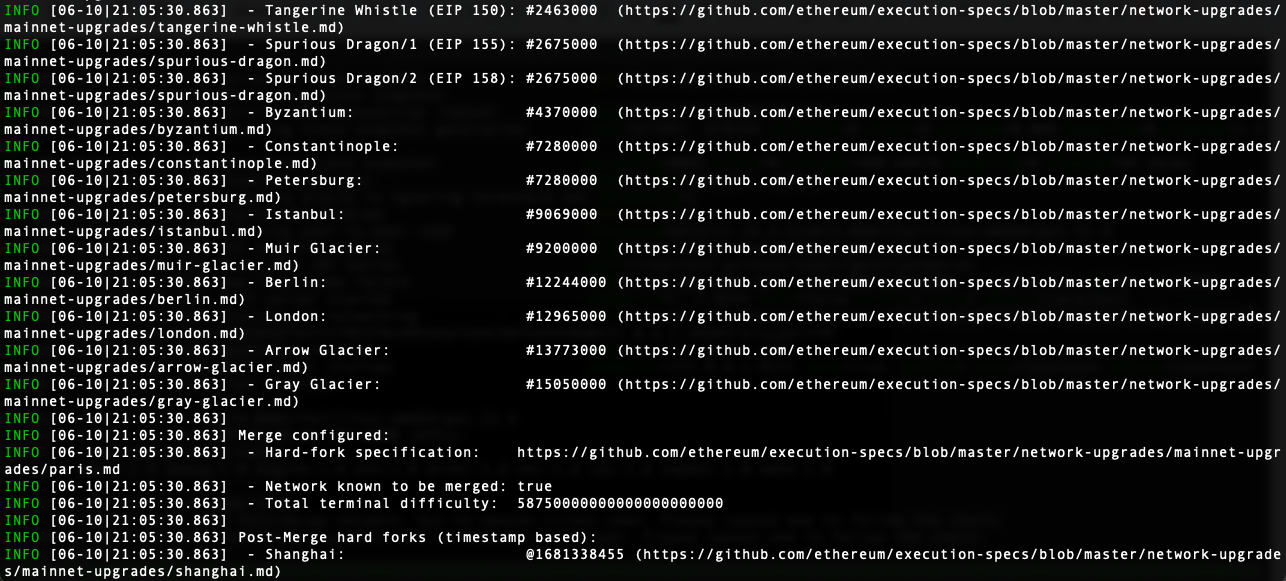
\includegraphics[scale=0.35]{IMAGES/launch22.png}
        % \caption{Количество круговых диаграмм, похожих на Пэкмена}
        \label{fig_pacman}
\end{figure}

\begin{figure}[ht]
        \centering
        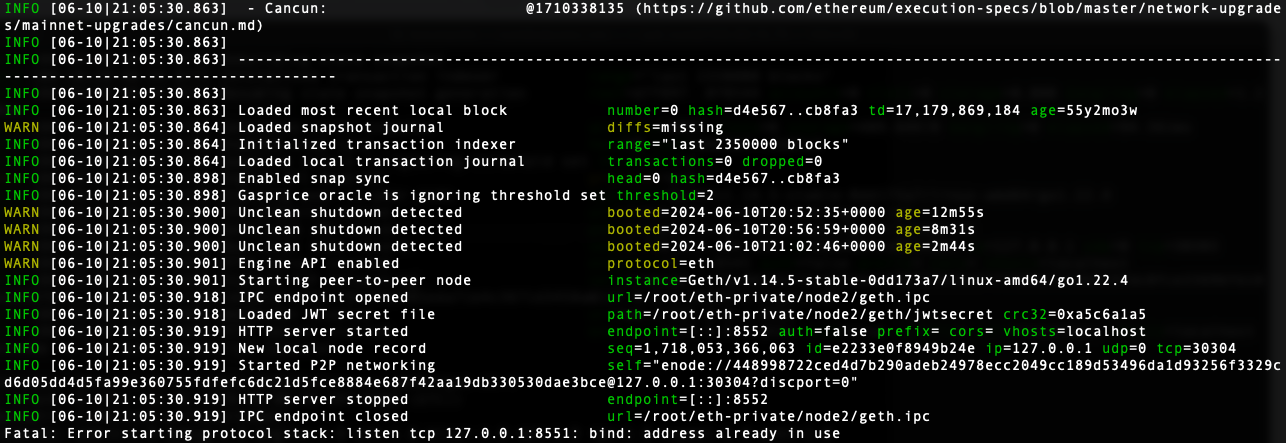
\includegraphics[scale=0.35]{IMAGES/launch23.png}
        % \caption{Количество круговых диаграмм, похожих на Пэкмена}
        \label{fig_pacman}
\end{figure}
\vspace{-0.75cm}
\newpage
Отримуємо помилку.

\vspace{0.65cm}
Спробуємо також просто запустити другу ноду, яка ніяк не залежить від першої:
\begin{verbatim}
geth --datadir ~/eth-private/node2 --http --http.addr "0.0.0.0" 
--http.port 8552 --http.api "eth,net,web3,personal" --nodiscover
--port 30304 console
\end{verbatim}

\vspace{-0.5cm}

\begin{figure}[ht]
        \centering
        
\includegraphics[scale=0.35]{IMAGES/errorLaunch2.png}
        % \caption{Количество круговых диаграмм, похожих на Пэкмена}
        \label{fig_pacman}
\end{figure}
\vspace{-0.5cm}
Бачимо, що отримуємо помилку аналогічну першому випадку.

\section{Тестування операцій в приватній ноді}

Спробуємо в запущеній першій ноді перевірити її стан:
\begin{verbatim}
eth.syncing
\end{verbatim}

\vspace{-0.5cm}

\begin{figure}[ht]
        \centering
        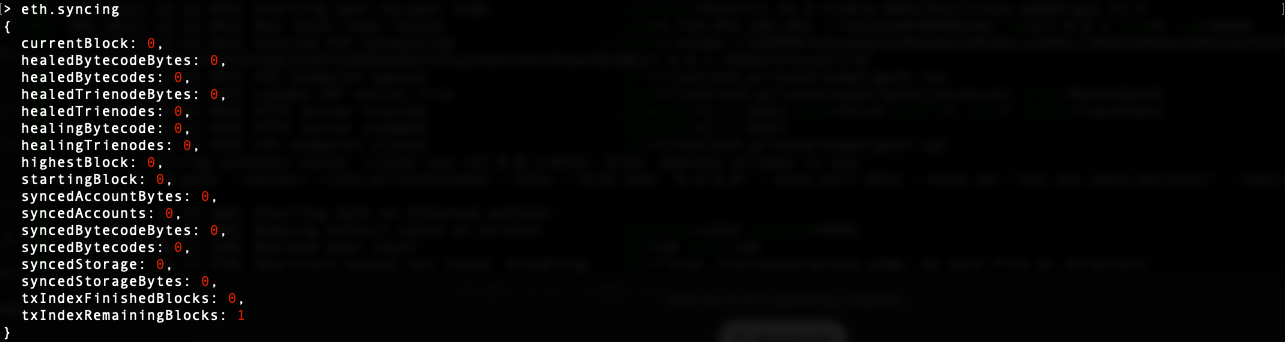
\includegraphics[scale=0.35]{IMAGES/eth-syncing.png}
        % \caption{Количество круговых диаграмм, похожих на Пэкмена}
        \label{fig_pacman}
\end{figure}
\vspace{-0.75cm}
\begin{verbatim}
eth.blockNumber
\end{verbatim}

\vspace{-0.5cm}

\begin{figure}[h!]
        \centering
        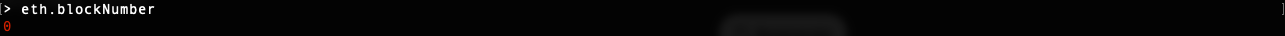
\includegraphics[scale=0.35]{IMAGES/eth-blockNumber.png}
        % \caption{Количество круговых диаграмм, похожих на Пэкмена}
        \label{fig_pacman}
\end{figure}

Спробуємо перевірити стан майнінгу ноди:
\begin{figure}[ht]
        \centering
        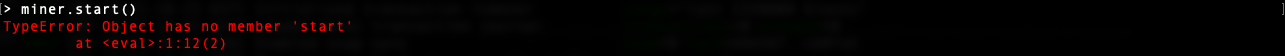
\includegraphics[scale=0.35]{IMAGES/minerError.png}
        % \caption{Количество круговых диаграмм, похожих на Пэкмена}
        \label{fig_pacman}
\end{figure}

А також перевіримо можливість переведення ETH між акаунтами:
\begin{figure}[ht]
        \centering
        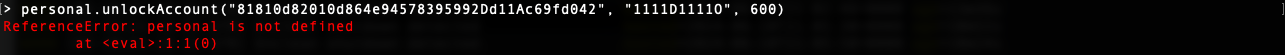
\includegraphics[scale=0.35]{IMAGES/unlockAccError.png}
        % \caption{Количество круговых диаграмм, похожих на Пэкмена}
        \label{fig_pacman}
\end{figure}
\vspace{-1.25cm}
\begin{figure}[ht]
        \centering
        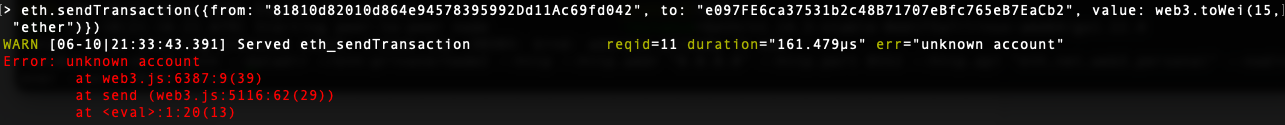
\includegraphics[scale=0.35]{IMAGES/sendTxError.png}
        % \caption{Количество круговых диаграмм, похожих на Пэкмена}
        \label{fig_pacman}
\end{figure}

В обох випадках отримали відмову перевірки, оскільки не був запущений майнінг для даної ноди, а відповідно -- недоступні будь-які операції.


При спробі виконати команду запуску ноди з майнінгом з оператором \texttt{--miner.threads}:
\begin{verbatim}
geth --datadir ~/eth-private-node/node1 --http --http.addr "0.0.0.0" 
--http.port 8545 --http.corsdomain "*" --http.api personal,eth,net,
web3,miner --mine --miner.threads 1 --networkid 1337
--allow-insecure-unlock
\end{verbatim}

А також при спробі ж виконати команду запуску ноди – з оператором \texttt{--miner.etherbase}:
\begin{verbatim}
geth --datadir ~/eth-private-node/node1 --networkid 1337 --http 
--http.addr "0.0.0.0" --http.port 8545 --http.corsdomain "*" 
--http.api personal,eth,net,web3,clique --allow-insecure-unlock 
--nodiscover --mine --miner.etherbase "81810d8201...Dd11Ac69fd042" 
--unlock "81810d8201...Dd11Ac69fd042" 
--password /root/eth-private-node/.. --verbosity 3 console
\end{verbatim}

\newpage
В обох випадках отримували помилку:
\begin{figure}[h!]
        \centering
        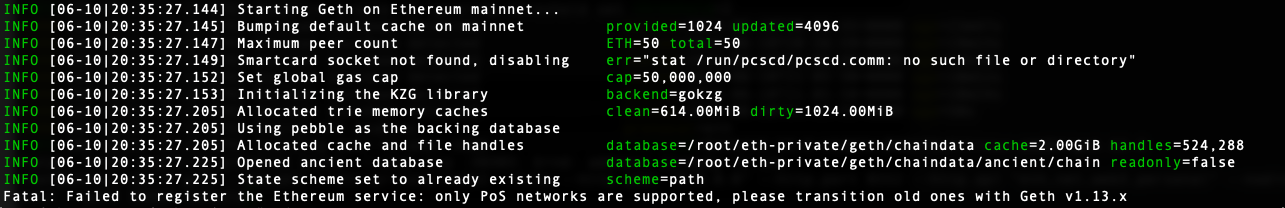
\includegraphics[scale=0.35]{IMAGES/onlyPoSError.png}
        % \caption{Количество круговых диаграмм, похожих на Пэкмена}
        \label{fig_pacman}
\end{figure}

Крім цього, пробували запуск та налаштування власної ноди Ethereum на протоколі PoA (Proof-Of-Authority), де отримували аналогічну помилку про недоступність Geth до відмінних від PoS протоколів.

\chapconclude{\ref{chap:review}}

Отже, наразі більшість функціоналу Geth для PoW є застарілою, оскільки майнінг був вимкнений при переході на Ethereum 2.0 на Proof-Of-Stake. А PoS потребує більш складних зусиль (включно зі смарт-контрактом для стейкінгу) для коректного налаштування та роботи приватної ноди Ethereum.